% Options for packages loaded elsewhere
\PassOptionsToPackage{unicode}{hyperref}
\PassOptionsToPackage{hyphens}{url}
%

\documentclass[10pt]{ctexart}
\usepackage{lmodern}
\usepackage{float}
\usepackage[margin=2.3cm]{geometry}
\usepackage{fancyhdr}
\usepackage{tikz}

\usepackage{amssymb, amsmath}
\usepackage{ifxetex, ifluatex}
\usepackage{xcolor}
\IfFileExists{xurl.sty}{\usepackage{xurl}}{} % add URL line breaks if available
\IfFileExists{bookmark.sty}{\usepackage{bookmark}}{\usepackage{hyperref}}
\hypersetup{
  hidelinks, 
  pdfcreator={LaTeX via pandoc}}
\urlstyle{same} % disable monospaced font for URLs
\usepackage{graphicx}
\makeatletter
\def\maxwidth{\ifdim\Gin@nat@width>\linewidth\linewidth\else\Gin@nat@width\fi}
\def\maxheight{\ifdim\Gin@nat@height>\textheight\textheight\else\Gin@nat@height\fi}
\makeatother
% Scale images if necessary,  so that they will not overflow the page
% margins by default,  and it is still possible to overwrite the defaults
% using explicit options in \includegraphics[width,  height,  ...]{}
\setkeys{Gin}{width=\maxwidth, height=\maxheight, keepaspectratio}
% Set default figure placement to htbp
\makeatletter
\def\fps@figure{htbp}
\makeatother
\setlength{\emergencystretch}{3em} % prevent overfull lines
\providecommand{\tightlist}{%
  \setlength{\itemsep}{0pt}\setlength{\parskip}{0pt}}
\setcounter{secnumdepth}{-\maxdimen} % remove section numbering

\author{}
\date{}

\pagestyle{fancy} 
\fancyhead[L]{\it《宏观经济学》}
\fancyhead[R]{\it 数字经济专业}

\fancyfoot[R]{\thepage}
\fancyfoot[C]{\it 授课教师:雷浩然}
\fancyfoot[L]{\it 湖南大学课程}


\begin{document}

\section{总供给理论}

\begin{itemize}
\item
  向下倾斜的总需求 (AD) 曲线, 说明了价格水平的上升会降低均衡产出. 总需求曲线由 IS-LM 模型推导而来. 
\item
  本章的重难点是总供给 (AS) 曲线, 它在长期和短期中的表现完全不同. 
  本讲义顺序如下:

  \begin{enumerate}
  \def\labelenumi{\arabic{enumi}.}
  \item
    首先, 分别讨论长期总供给 (LRAS, Long Run Aggregate Supply) 和(极端) 短期情形的总供给.
  \item
    然后, 讨论经济如何从短期均衡过渡到长期均衡.
  \item  
    最后, 在``名义工资只能上升、不能下降''的假设下, 推导一般情况下的总供给曲线.
  \end{enumerate}
\end{itemize}

\paragraph{长期均衡:古典情形}
\begin{itemize}
\item
  长期中, 由于价格可以灵活变动, 失业率和产出都处在\textbf{自然状态}.
  \begin{itemize}
  \item
    失业率:\textbf{自然失业率}
  \item
    GDP: \textbf{潜在 GDP} (也叫\textbf{潜在产出}, 或\textbf{自然产出})
  \end{itemize}
\item
  原因: 劳动力市场的名义工资 $W$ 会根据价格水平 $P$
  的变化进行调整, 使劳动市场维持在``充分就业''状态
\end{itemize}

\begin{itemize}
\item
  经济体的产出由\textbf{生产函数}决定. 生产函数形式为 \(Y = F(K, L)\), 其中
  \begin{itemize}
    \item
      $Y$ 表示产出, 即实际 GDP
    \item
      $K$ 表示用于生产的资本, 如厂房、生产设备等
    \item
      $L$ 表示劳动力
    \item
      $F$ 是一个函数, 它的输入是
      资本 $K$ 和劳动力 $L$,  输出是产出 $Y$.
    \end{itemize}
\item
  由于劳动力处于充分就业状态, $L$ 为常数: \(L = \bar L\)
\item
  假定资本 $K$ 和生产函数 $F$ 也不变, 因此 $Y$ 也不变: \(Y = \bar Y\)

  \begin{itemize}
  \item
    \(\bar Y\) 就是课程第一章里定义的潜在 GDP (潜在产出)
  \end{itemize}
\item
  \textit{结论}:长期的总供给曲线(LRAS,  \textit{Long-Run Aggregate Supply})是竖直的

  \begin{itemize}
  \item
    对任意价格水平 $P$,  均衡产出都为 \(\bar Y\)
  \end{itemize}
\item 这一结论有以下两个推论:
  \begin{enumerate}
    \item  在长期均衡中, 总需求的变化不影响均衡产出, 只影响均衡价格
    \item  长期中货币是中性的. 以图 \ref{fig:money-neutral} 为例, 央行降低货币供给, 导致总需求从 $AD_1$ 下降到 $AD_2$,  均衡从点 A
    移动到点 B. 均衡价格下降, 但产出始终为 $\bar Y$
  \end{enumerate}






\begin{figure}
\centering
\begin{tikzpicture}
\tikzstyle{every node}=[font=\footnotesize] 

\draw[<->] (0, 5) -- (0, 0) -- (5, 0);
    \node[left] at (0, 5) {价格水平, $P$};
    \node[below] at (6, 0) {收入/产出, $Y$};
\draw[] (3, 0) -- (3, 4.5); % LRAS
    \node[below] at (3, 0) {$\bar Y$};
    \node[above] at (3, 4.6) {\textit{LRAS}};


\draw[] (1, 5) to [out=300, in=150] (5, 2); % AD1
    \node[right] at (5, 2) {$AD_1$};

\draw[] (1, 3.5) to [out=300, in=150] (5, 1); % AD2
    \node[right] at (5, 1) {$AD_2$};

\draw[fill] (3, 3.05) circle [radius=1pt];
    \node[right] at (3, 3.15) {$A$}; 
\draw[dotted] (0, 3.05) -- (3, 3.05); %A
    \node[left] at (0, 3.05) {$P_1$}; 

\draw[fill] (3, 1.88) circle [radius=1pt];
    \node[right] at (3, 1.95) {$B$}; 
\draw[dotted] (3, 1.88) -- (0, 1.88); %B
    \node[left] at (0, 1.88) {$P_2$};

\end{tikzpicture}
\caption{长期中的``货币中性''现象}
\label{fig:money-neutral}
\end{figure}

  
\end{itemize}

\paragraph{货币中性} $\quad$
  长期均衡中, 央行增发货币只会使价格水平 $P$ 和工资 $W$
  等比例地变化, 通货膨胀会\textit{均匀地}作用在所有价格上, 产出 $Y$ 不变.

  \begin{itemize}
  \item
    这个现象被称为\textbf{货币中性} (neutrality of
    money). 它的另一种表述如下: 长期内货币供给的变化只会影响名义量 (名义价格$P$,  名义工资$W$,  名义货币余额 $M$, ...), 
    而不能影响实际量 (产出 $Y$,  消费 $C$,  实际货币余额\({M} \over {P}\),  实际工资$W \over P$, 失业率, ...)
\end{itemize}

\paragraph{极端短期情形}

\begin{itemize}
\item
  极端短期情形的总供给(SRAS,  \textit{Short-Run Aggregate Supply})曲线是水平的.
  \begin{itemize}
  \item
    给定价格水平 $P$, 均衡产出由过 P 的水平线和 AD 的交点决定
  \item
    均衡产出完全由总需求 (AD) 决定
  \end{itemize}
\item
  在短期均衡中, 总需求的变化会影响均衡产出. 

  \begin{itemize}
  \item
    图 \ref{fig:sr} 中, 央行降低货币供给导致总需求下降. 由于此时总供给线是水平的, 短期内价格水平不变, 产出下降.
  
  \begin{figure}[H]
\centering
\includegraphics[width=0.6\textwidth]{/Users/lhr45678/articles/book-mit6001x-2021/SR-down.jpg}
\caption{短期内货币非中性}
\label{fig:sr}
\end{figure} 
  \end{itemize}
  
  \item
    \textit{``货币非中性''的文字阐释:} 虽然总需求因``货币供给减少''而下降, 但价格没有调整, 企业被黏在过高的价格上. 这导致企业卖出的产品下降. 企业因此减少生产并解雇工人, 经济面临衰退.   
\end{itemize}



\paragraph{短期均衡过渡到长期均衡:价格调整情形} $\, $

我们以图3为例, 考虑当经济体偏离长期均衡时, 是如何随着价格调整, 由短期均衡逐渐移动到长期均衡的. 

短期内:

\begin{itemize}
  \item
    若价格水平固定在 \(P_1\),  均衡为点 \(K\)
  \item
    若价格水平固定在 \(P_2\),  均衡为点 \(C\)
\end{itemize}

长期中:

  \begin{itemize}
  \item
    对任意 \(P\), 产出均为自然水平 \(\bar Y\)
  \item 长期均衡为点 \(C\), 
    长期均衡价格为 \(P_2\)
  \end{itemize}

假设现在的价格水平是 \(P_1\), 随着时间流逝:
  \begin{itemize}
  \item
    经济体会由短期均衡 \(K\) 沿着 AD 曲线移动到长期均衡 \(C\)
  \item
    价格水平也会从 \(P_1\) 下降到 \(P_2\)
  \end{itemize}


\bigskip

\begin{figure}
\centering
\begin{tikzpicture}
\usetikzlibrary{arrows.meta}
\tikzstyle{every node}=[font=\footnotesize] 

\draw[<->] (0, 5) -- (0, 0) -- (5, 0);
    \node[left] at (0, 5) {价格水平, $P$};
    \node[below] at (6, 0) {收入/产出, $Y$};
\draw[] (3, 0) -- (3, 4.5); % LRAS
    \node[below] at (3, 0) {$\bar Y$};
    \node[above] at (3, 4.6) {\textit{LRAS}};


%\draw[] (1, 3.5) to [out=300, in=150] (5, 1); % AD
%    \node[right] at (5, 1) {$AD$};

\draw[fill] (1, 3) circle [radius=1.5pt];
    \node[right] at (1.1, 3.15) {$K$}; 
\draw[] (0, 3) -- (5, 3); %A
    \node[left] at (0, 3) {$P_1$}; 
    \node[right] at (5, 3) {\textit{SRAS}$_1$}; 



\draw[-{>[scale=2.5, 
          length=3, 
          width=6]}, line width=0.4pt] (1, 3) -- (2, 2.25); 

\draw[] (0.5, 3.375) -- (1, 3) -- (3, 1.5) -- (4, 0.75) node [right] {$AD$} ; %AD

\draw[fill] (3, 1.5) circle [radius=1.5pt];
    \node[right] at (3, 1.65) {$C$}; 
\draw[] (5, 1.5) -- (0, 1.5); %B
    \node[left] at (0, 1.5) {$P_2$};
    \node[right] at (5, 1.5) {\textit{SRAS}$_2$}; 
    
\end{tikzpicture}
\caption{短期均衡$K$到长期均衡$C$}

\end{figure}


\clearpage

\paragraph{短期均衡过渡到长期均衡:需求冲击情形 (Demand Shock)}


\begin{itemize}
\item
  假设经济体开始时处于长期均衡中, 此时央行决定增加货币供给. 
\item
  如图4所示, 总需求曲线从 $AD_1$ 上移到 $AD_2$. 
\item
  短期内, 价格是黏性的, 均衡从 A 水平移动到 B
  \begin{itemize}
  \item
    产出和就业率超出自然水平, 经济迎来繁荣
  \end{itemize}
\item
  随着时间流逝, 由于需求高涨, 工资和商品价格开始上升
\item
  价格水平的调整, 使经济沿着总需求曲线移动到点 C,  达到新的长期均衡

  \begin{itemize}
  \item
    新的均衡中, 产出和就业又回到自然水平, 但价格比之前的长期均衡 (C)
    更高
  \end{itemize}
\item 结论:
  \begin{itemize}
  \item 总需求的扩张会在短期内提高产出. 
  \item 但随着时间流逝, 价格和工资不断调整, 产出会回到自然水平
  \end{itemize}

  
\end{itemize}

\begin{figure}
\centering
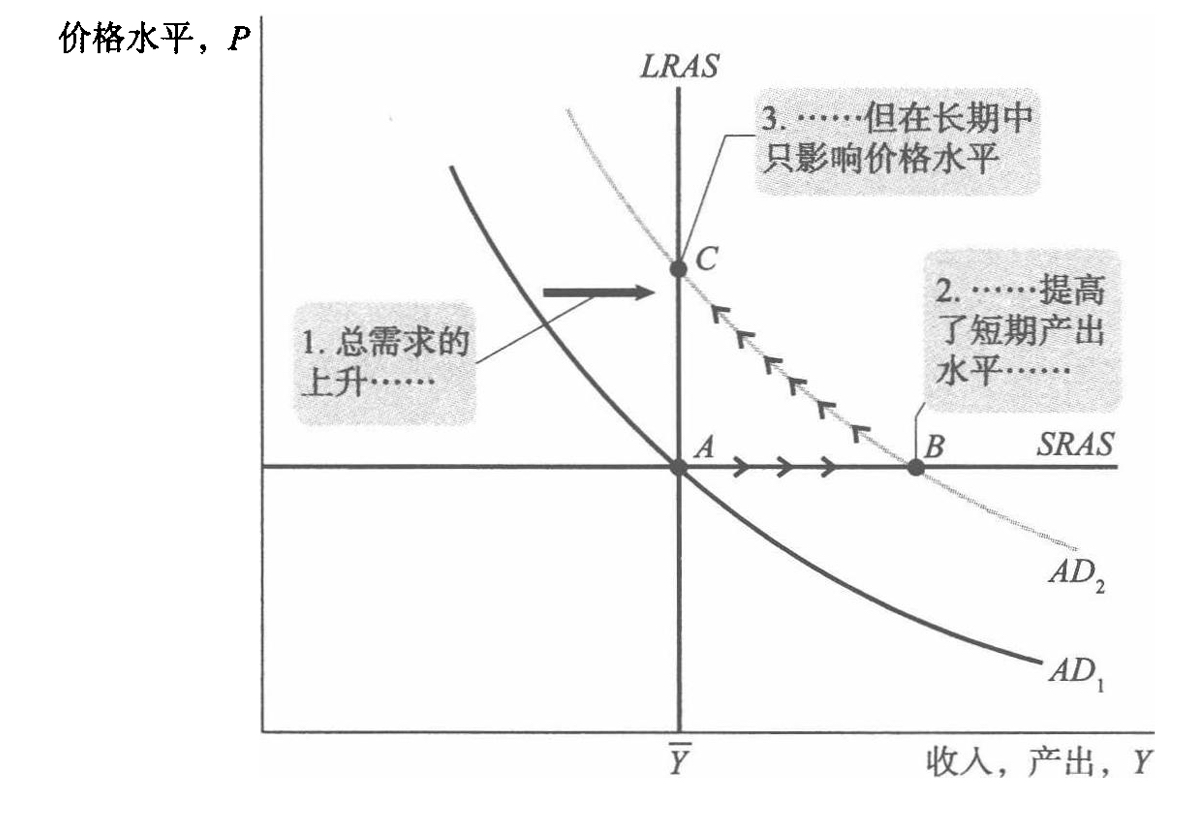
\includegraphics[width=0.55\textwidth]{/Users/lhr45678/Dropbox/hnu-macro-2021/fig/supply-shock.jpeg}
\caption{总需求上升}
\end{figure}



\paragraph{货币对均衡的影响}


\begin{itemize}
\item
  长期内, 货币是中性的:货币供给的变动只会导致通货膨胀, 不影响产出.
\item
  短期内, 货币是非中性的:货币供给的变动对产出有实际影响.
\end{itemize}

十八世纪英国哲学家兼经济学家休谟 (David Hume)
在《论货币》一书中这样描述金银供给增加对当时英国经济的影响:

\begin{quote}
\it ...
尽管商品的高价是金银增加的一个必然后果, 但这并不是在金银增加后立刻发生的;而是经过一段时间后, 当增加的货币在各地被用于交易, 其效应才为社会各阶层人士所察觉. 首先, 人们没有察觉任何变化;慢慢地, 价格开始上涨, 先是商品一, 然后是商品二;直到最后, 总体价格达到了与新的流通金银相适应的水平. 
\end{quote}

\paragraph{如何``称呼'' LRAS 和 SRAS}
\begin{itemize}
\item 
  目前为止, 两种情形的总供给曲线的推导本身十分简单.
\item
  马工程教材在不同的地方, 使用不同的名字称呼总供给的两种情形, 如: P121,
  ``凯恩斯主义萧条情况下的总供给''和``古典的长期稳定情况下的总供给'';P123,
  ``极端的短期模型''或``萧条模型'', 以及``极端的长期模型'';P124,
  ``古典情况的 AD-AS 模型''; 等等...
\item  
  这给初学者带来了不必要的困扰. 我们不妨便宜行事:
  \begin{itemize}
\item
  ``水平的总供给曲线''称为(极端)短期情形, 或凯恩斯情形, 或萧条情形.
\item
  ``竖直的总供给曲线''称为长期情形, 或古典情形.
\item
  后文会介绍``向上方倾斜的总供给曲线'', 
  我们遵循教材称它为一般情形. 但是, 有时习题也会把它称为短期情形, 请同学们注意分辨.
  \end{itemize}
\end{itemize}


\hypertarget{header-n2318}{%
\paragraph{小结}\label{header-n2318}}

\begin{itemize}
\item
  目前为止, 我们的经济体可由三个方程描述. 其中两个是
  \[Y = C(Y-T) + I(r) + G \tag{IS}\]
  \[\frac{M}{P} = L(r, Y) \tag{LM}\]
\item
  它包含了三个内生变量: \(Y\),  \(P\) 和 \(r\). 由IS 和 LM 可推导 AD 曲线. 
\item
  凯恩斯主义固定了价格. 它的第三个方程是
  \[P = P_1  \tag{短期均衡条件}\]
\item
  古典方法固定了产出, 允许价格自由调整使得市场达到自然状态, 它的第三个方程是
  \[Y=\bar Y \tag{长期均衡条件} \]
\item
  随着时间的流逝, 经济体会从短期均衡逐渐过渡到长期均衡状态. 
\end{itemize}

\paragraph{一般情形:向上倾斜的AS}
\begin{itemize}
\item
  目前为止, 我们学习了
  \begin{enumerate}
    \item 长期总供给曲线 (LRAS) 是竖直的:产出固定在自然水平 $\bar Y$
    \item 极端短期总供给曲线 (SRAS) 是水平的:价格水平固定在某个 $P_0$
  \end{enumerate}
\item
  这是我们的分析起点. 这两条曲线的逻辑很简单, 其差别在于价格是否能自由变动. 
\item
  实际中, 许多价格在短期内具有黏性, 难以改变(如工资);
\item   
  但也存在一些价格能对环境的变化迅速作出调整, 如淘宝、京东等网店的标价. 
\item
  如果允许某些价格能部分变动, 就可以推导出
  向上倾斜的总供给曲线. 这类 AD 曲线有很多种推导方法, 
  这里我们介绍``刚性工资''下的推导.
  \begin{itemize}
  \item
    \textbf{刚性工资:} 名义工资 W 只能升, 不能降.
  \item
    可类比消费函数理论中的``棘轮效应''理解.
  \end{itemize}
\item
  模型的主要逻辑如下. 假设初始时经济处于长期均衡中, 价格水平为
  \(P_0\), 产出为 $Y_0$, 名义工资为 \(W\), 就业人数为 $N$.   \begin{enumerate}
  \def\labelenumi{\arabic{enumi}.}
  \item
    若价格水平从 $P_0$上升到 \(P_1\) (见图5): 
    \begin{itemize}
    \item 此时工人的实际工资
    \(W/P_1\) 下降, 劳动市场的供给小于需求
    \item
      名义工资会迅速作出调整, 上升到 \(W_1\), 使得实际工资\(W_1/P_1( = W/P_0)\) 不变, 
      均衡时就业人数仍为 \(N\),  因此产出不变
    \item 由于此时工资可自由上升, 类比古典情形理解可知, 此处 AS 是竖直的  
    \end{itemize}
  \item
    若价格水平下降到 \(P_2<P_0\). 此时工人的实际工资
    \(W/P_2\) 上升, 劳动市场的供给大于需求. 

    \begin{itemize}
    \item
      但由于``工资刚性'', 名义工资 $W$ 无法下降. 
    \item  
      面对高昂的用工成本, 企业会减少员工数量, 均衡时就业人数下降至 $N_2 < N$, 产出下降至 $Y_2$.
    \end{itemize}
  \item
    总结:

    \begin{itemize}
    \item
      价格高于初始水平 \(P_0\)
      时, 名义工资可上升, 此时总供给曲线竖直(对应价格可自由变动的古典情形). 
    \item
      价格低于初始水平 \(P_0\)
      时, 名义工资无法下降、只能维持不变. 此时实际工资上升, 这导致就业人数下降, 产出下降. 
    \end{itemize}
  \end{enumerate}
  \begin{figure}\centering
\begin{tikzpicture}
  \tikzstyle{every node}=[font=\footnotesize] 
  \draw[<->] (0, 5) -- (0, 0) -- (5, 0);
    \node[left] at (0, 5) {价格水平, $P$};
    \node[below] at (6, 0) {收入/产出, $Y$};

  \draw[thick] (1, 1) to [out=30, in=-120] (4, 3);
  \draw[thick] (4, 5) -- (4, 3); 
    \node[right] at (4, 5) {$AS$};
 
  \draw[dotted] (4, 3) -- (4, 0); 
    \node[below] at (4, 0) {$Y_0$};

  \draw[dotted] (4, 3) -- (0, 3); 
    \node[left] at (0, 3) {$P_0$};

  \draw[dotted] (4, 4) -- (0, 4); 
    \node[left] at (0, 4) {$P_1$};
 
   \draw[dotted] (3, 2) -- (3, 0); 
    \node[below] at (3, 0) {$Y_2$}; 
 
   \draw[dotted] (3, 2) -- (0, 2); 
    \node[left] at (0, 2) {$P_2$};  
 
\end{tikzpicture}
\caption{一般情形下的总供给曲线}  
\end{figure}

\item 
  教材还介绍了所谓倒 L 型总供给, 作为图5所示的一般总供给线的简化. 这个倒 L 型曲线了解即可, 实际分析中基本用不上, 我们只会用到长期、极端短期和一般情形下的总供给曲线.
\end{itemize}
\end{document}
